\documentclass{article} % Defines the document class, article is commonly used

\usepackage{amsmath}    % Allows for more advanced math formatting
\usepackage{amssymb}    % Provides additional mathematical symbols
\usepackage{amsthm}     % \qed
\usepackage{graphicx}   % image
\usepackage{float}      % image placement
\usepackage{hyperref}
\hypersetup{
    colorlinks=true,       % false: boxed links; true: colored links
    linkcolor=black,       % color of internal links
}
\usepackage[margin=1.5in]{geometry}

\begin{document}

\title{EEC133 - Radiation Fundamentals and Basic Antennas}
\author{Tao Wang}
\date{\today}

\maketitle
\tableofcontents

\section{Spherical Coordinate}
\begin{quote}
    A position in spherical coordinate is characterized by $R, \space \theta, \space \phi$.
    An infinitesimal surface area patch, $dA$, is $dA = R^2 \sin(\theta) \space d\theta d\phi$.
    \smallskip

    $d\Omega = \sin(\theta) d\theta d\phi$ is defined as the \textbf{solid angle}.
    Therefore, $R^2 d\Omega$ is the infinitesimal surface area patch.
\end{quote}
\begin{figure}[H]
    \centering
    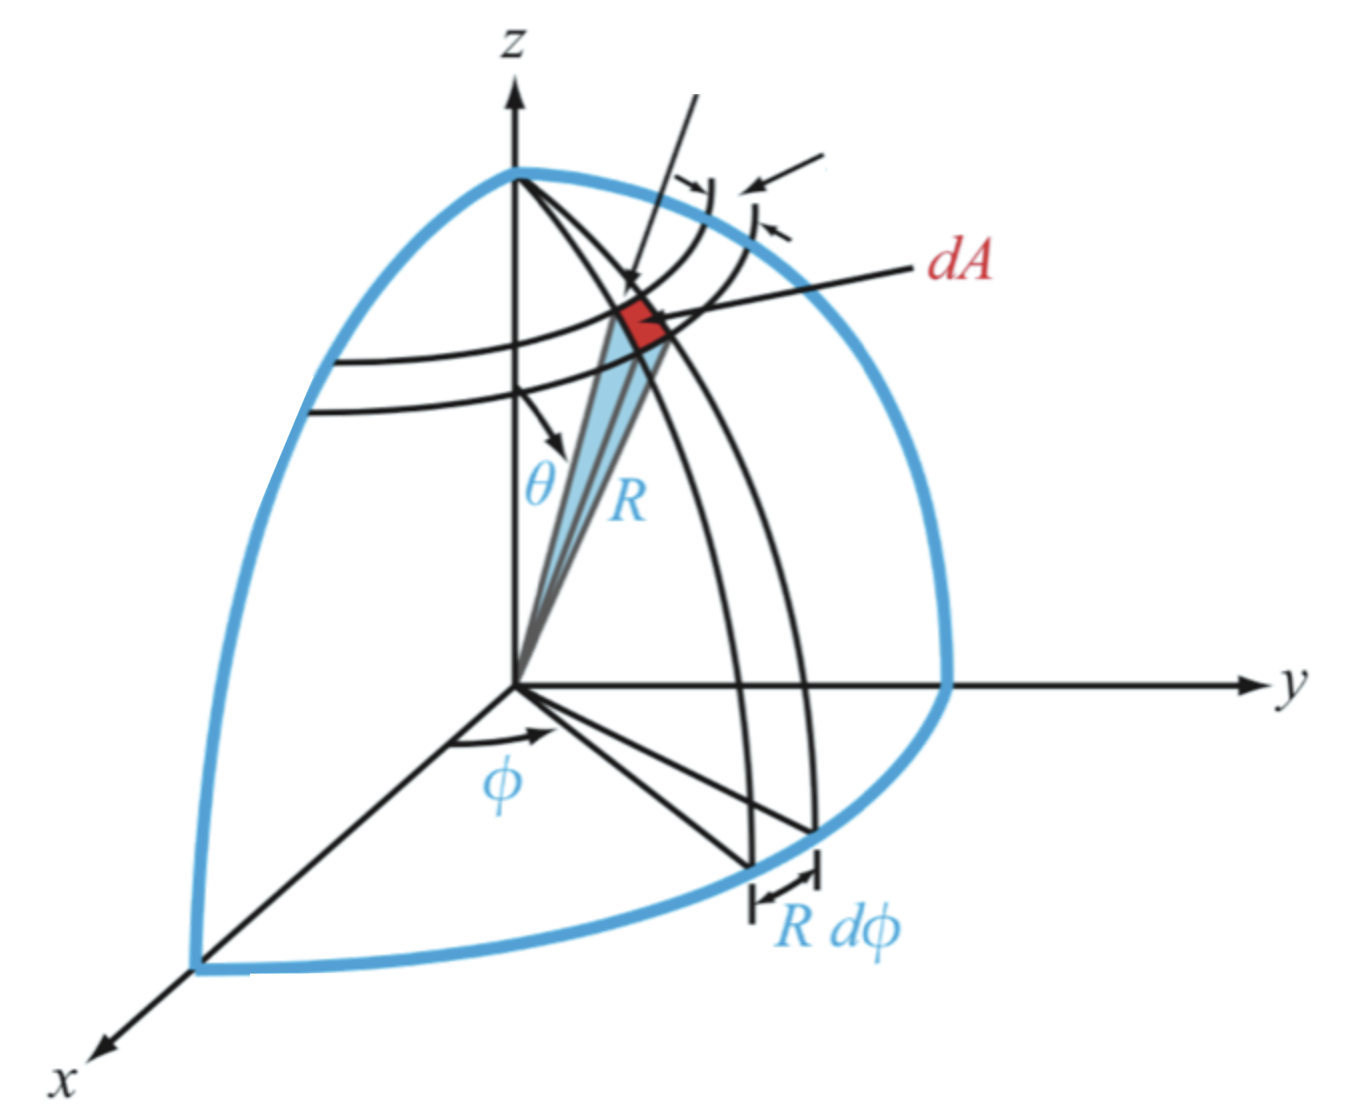
\includegraphics[width=0.8\textwidth]{./image/figure1.png}
    \caption{Spherical Coordinate}
\end{figure}

\section{Radian and Steradian}
\begin{itemize}
    \item \textbf{Radian}: measure of \textit{angle}. $s = r \theta$, where $s$ is the arc length, $r$ is the radius, and $\theta$ is the angle in radian.
    \item \textbf{Steradian}: measure of \textit{solid angle}. $A = r^2 \Omega$, where $A$ is the surface area patch, $r$ is the radius, and $\Omega$ is the solid angle.
\end{itemize}

\section{Properties of Antenna Wave}
\begin{quote}
    The wave propagates spherically according to the Maxwell's Equations. Moreover, we could approximate the radiated wave to be a plain wave because the wavefront looks flat and field is approximately constant.
\end{quote}
\begin{figure}[H]
    \centering
    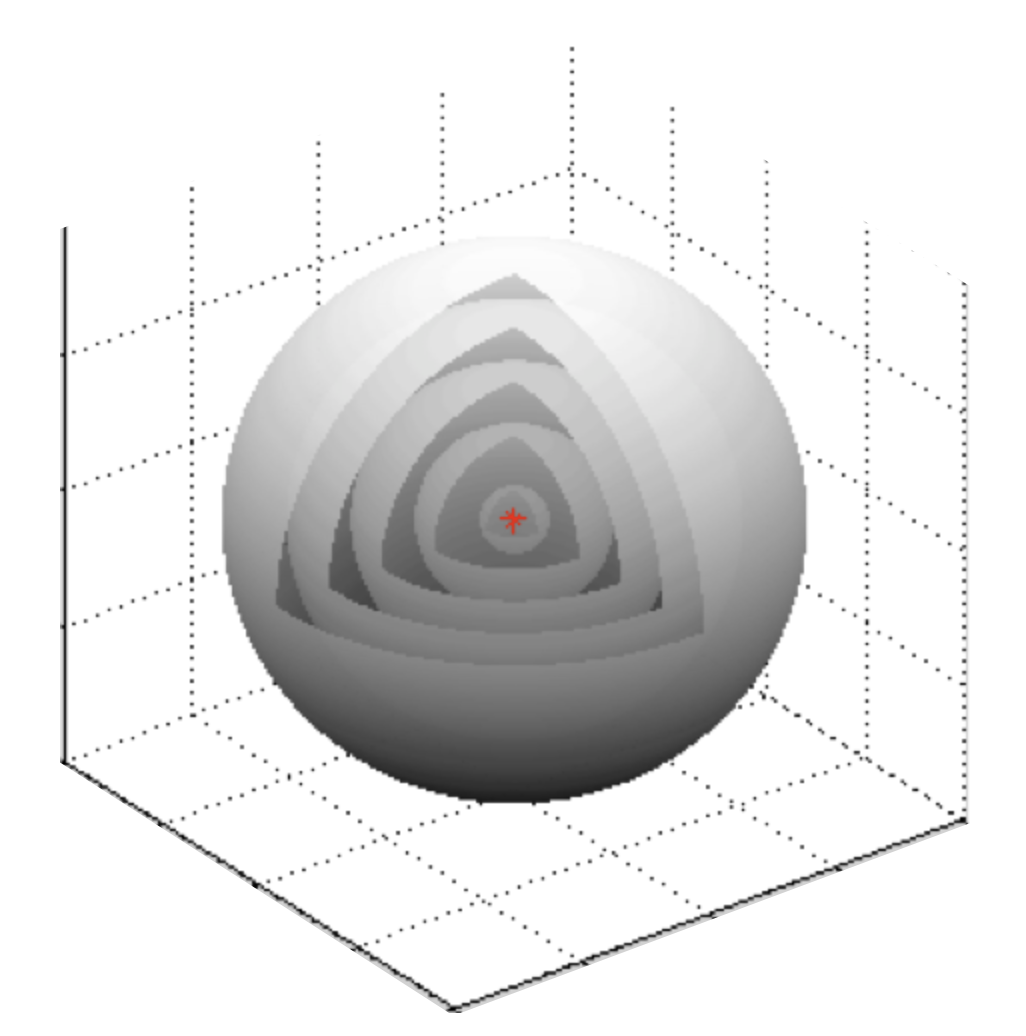
\includegraphics[width=0.6\textwidth]{./image/figure2.png}
    \caption{Spherical Electromagnetic Disturbances}
\end{figure}
\subsection{Power Carried By the Wave}
\begin{quote}
    The Poynting vector associated with the wave traveling in a lossless medium:
    \[\vec{S}_{av} = \hat{r} S(r, \theta, \phi) = \hat{r} f(r) U(\theta, \phi)\]
    where $U(\theta, \phi)$ is the \textbf{Radiation Intensity}.
    \smallskip
    We can find the total power by integrating the Poynting Vector over the surface area.

    \[P(r) = \int_{\text{Sphere}} \vec{S}_{av} \cdot d\vec{A}\]
    \[= \int_{0}^{2\pi} \int_{0}^{\pi} \hat{r} f(r)U(\theta, \phi) \cdot \hat{r} r^2 \sin(\theta) d\theta d\phi\]

    We don't need to integrate the Poynting Vector over the radius because the wave can only be at one radial distance away from the center at a given time.

    Since the integral doesn't depend on $r$, we have
    \[P(r) = f(r) r^2 \int_{0}^{2\pi} \int_{0}^{\pi} U(\theta, \phi) \sin(\theta) d\theta d\phi\]
    for simplicity, assume $f(r) = \frac{1}{r^2}$, then
    \[P(r) = \int U(\theta, \phi) d\Omega\]
    Therefore, the total radiated power is constant with $r$ due to the conservation of energy.

    Also, since total power = sum of Radiation Intensity $\times$ solid angle, the \textbf{Radiation Intensity is in Power per Steradian}.
\end{quote}

\subsection{Isotropic Radiator}
\begin{quote}
    The Isotropic Radiator is an antenna that radiates equally in all directions; The radiation intensity is the same for all direction. Then,
    \[U(\theta, \phi) = U_0\]

    Note,
    \[P_{rad} = \int U(\theta, \phi) d\Omega = U_0 \int d\Omega = U_0 4\pi\]
    Therefore,
    \[U_0 = \frac{P_{rad}}{4\pi}\]

    We can see that the unit of $U_0$ is $\frac{\text{Watts}}{\text{Steradian}}$.

\end{quote}

\section{Directivity}
\begin{quote}
    Since the radiation intensity, $U(\phi, \theta)$, is dependent of the total radiated power, we want to define another quantity that is independent of the radiated power.

    The \textbf{directivity pattern} of an antenna is the radiation intensity normalized by the radiation intensity of an isotropic radiator, which is
    \[D(\theta, \phi) = \frac{U(\phi, \theta)}{U_0} = 4 \pi \frac{U(\theta, \phi)}{P_{rad}}\]

    Notice that \[\int_{\text{sphere}}D(\theta, \phi)  d\Omega = 4 \pi\]

    Since $D(\theta, \phi) = U(\theta, \phi)(\frac{4\pi}{P_{rad}})$ and the sum of $D(\theta, \phi)$ is constant in one spherical shell, we know that \textbf{more radiation intensity in one direction means less in another} since they sum to a number.
    \bigskip

    We'll define another quantity, the \textbf{Directivity}, as
    \[D_0 = \max\{D_{\theta, \phi}(\theta, \phi)\}\]

    The directivity can also be written in terms of the normalized radiation intensity.

    \[D_0 = \frac{4 \pi}{\Omega_p} = \frac{4\pi}{\int_{\text{Sphere}} F(\theta, \phi) d\Omega}\]

    where $\Omega_p$ is the \textbf{pattern solid angle}. The smaller it is, the greater the directivity.

    The integral integrates the normalized radiation intensity, $F(\theta, \phi)$ over all direction from the sphere's center.

\end{quote}

\section{Beamwidth}

Beamwidth tells us how much the opening is for a lobe. A lobe is a region where radiation intensity is the highest.

\begin{figure}[H]
    \centering
    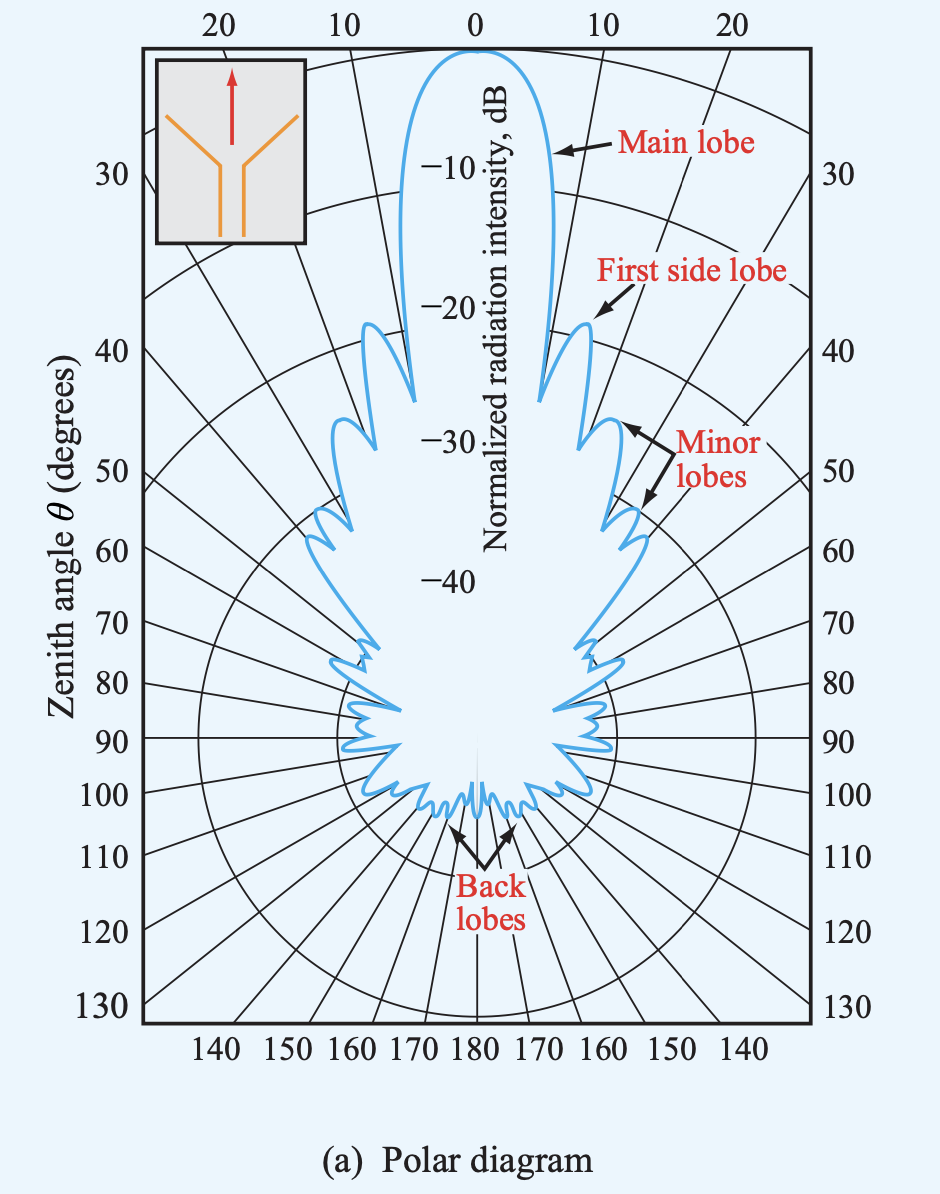
\includegraphics[width=0.5\textwidth]{./image/figure3.png}
    \caption{Polar Plot of Radiation Intensity}
\end{figure}

The half power beamwidth is

\[\theta_2 - \theta_1\]

where $\theta_2$ is the angle where the normalized radiation intensity is $\frac{1}{2}$.

It occurs at $\theta = \frac{\pi}{4}$ and $\theta = \frac{3\pi}{4}$.


\section{Antenna Parameters}
\begin{itemize}
    \item Radiation Intensity ($\frac{\text{Watts}}{\text{Steradian}}$): the amount of power radiated by the antenna to different directions.
          \[U(\theta, \phi)\]
    \item Normalized Radiation Intensity (Unitless)
          \[F(\theta, \phi) = \frac{U(\theta, \phi)}{U_{max}}\]
    \item Directivity Pattern ($\frac{1}{\text{Steradian}}$): the radiation intensity to different directions but normalized by a constant.
          \[D(\theta, \phi) = \frac{U(\theta, \phi)}{U_0} = 4 \pi \frac{U(\theta, \phi)}{P_{rad}}\]
    \item Directivity ($\frac{1}{\text{Steradian}}$):
          \[D_0 = \max\{D(\theta, \phi)\}\]
    \item Beamwidth (Steradian): the amount of opening where radiation intensity is the highest. Note that high directivity gives small beamwidth and vice versa.
          \[\Omega_A \approx \frac{4\pi}{D_0} \]
    \item Gain
          \[G_0 = \text{Efficiency} \times D_0\]
          where efficiency is $\frac{P_{rad}}{P_{in}}$
\end{itemize}

\section{Circuit Model of an Antenna}
\begin{figure}[H]2
    \centering
    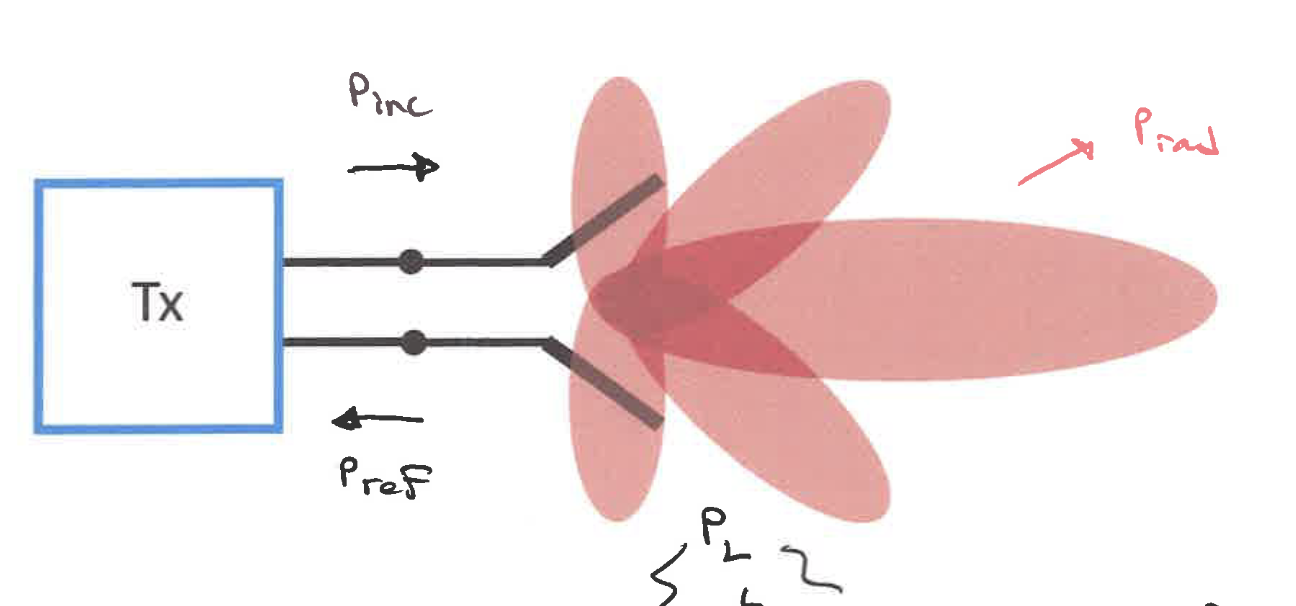
\includegraphics[width=0.5\textwidth]{./image/figure9.png}
    \caption{Circuit Model of an Antenna}
\end{figure}
\subsection{Power}
\begin{quote}
    Since the antenna dissipates power, radiate power, and reflects the transmitted power, we can model it as a load impedance that has resistance and reactance.
    \[Z_A = R_L + R_{rad} + j X_A\]

    We know that
    \[P_{in} = \frac{1}{2}|\tilde{I}|^2 (R_{rad} + R_L)\]

    Therefore,
    \[e = \frac{P_{rad}}{P_{in}} = \frac{\frac{1}{2}|\tilde{I}|^2 (R_{rad})}{P_{in} = \frac{1}{2}|\tilde{I}|^2 (R_{rad} + R_L)} = \frac{R_{rad}}{R_{rad} + R_L}\]
\end{quote}

\subsection{Optimizing $P_{in}$}

\begin{figure}[H]
    \centering
    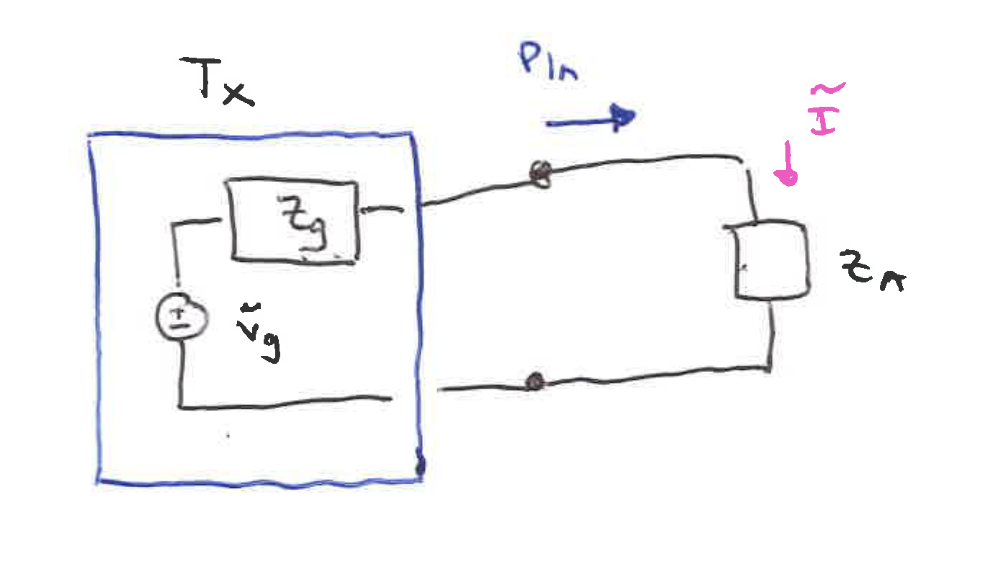
\includegraphics[width=0.5\textwidth]{./image/figure5.png}
    \caption{Thevenin Equivalent of Transmitter with Antenna as Load}
\end{figure}
\begin{quote}
    We can model the antenna as an impedance, $Z_A$, and the transmitted signal as a thevenin equivalent.

    Using some calculus, we will find that the maximum power is transferred to $Z_A$ when
    \[Z_g = Z_A^*\]

    When power is maximally transferred, $P_{in}$ is
    \[P_{in} = \frac{1}{2}|\tilde{I}|^2 R_A = \frac{1}{2}\left(\frac{|\tilde{V}_{TH}|}{2R_A}\right)^2R_A = \frac{|\tilde{V}_{TH}|^2}{8R_A}\]
\end{quote}

\subsection{Optimizing $P_{out}$}

\begin{figure}[H]
    \centering
    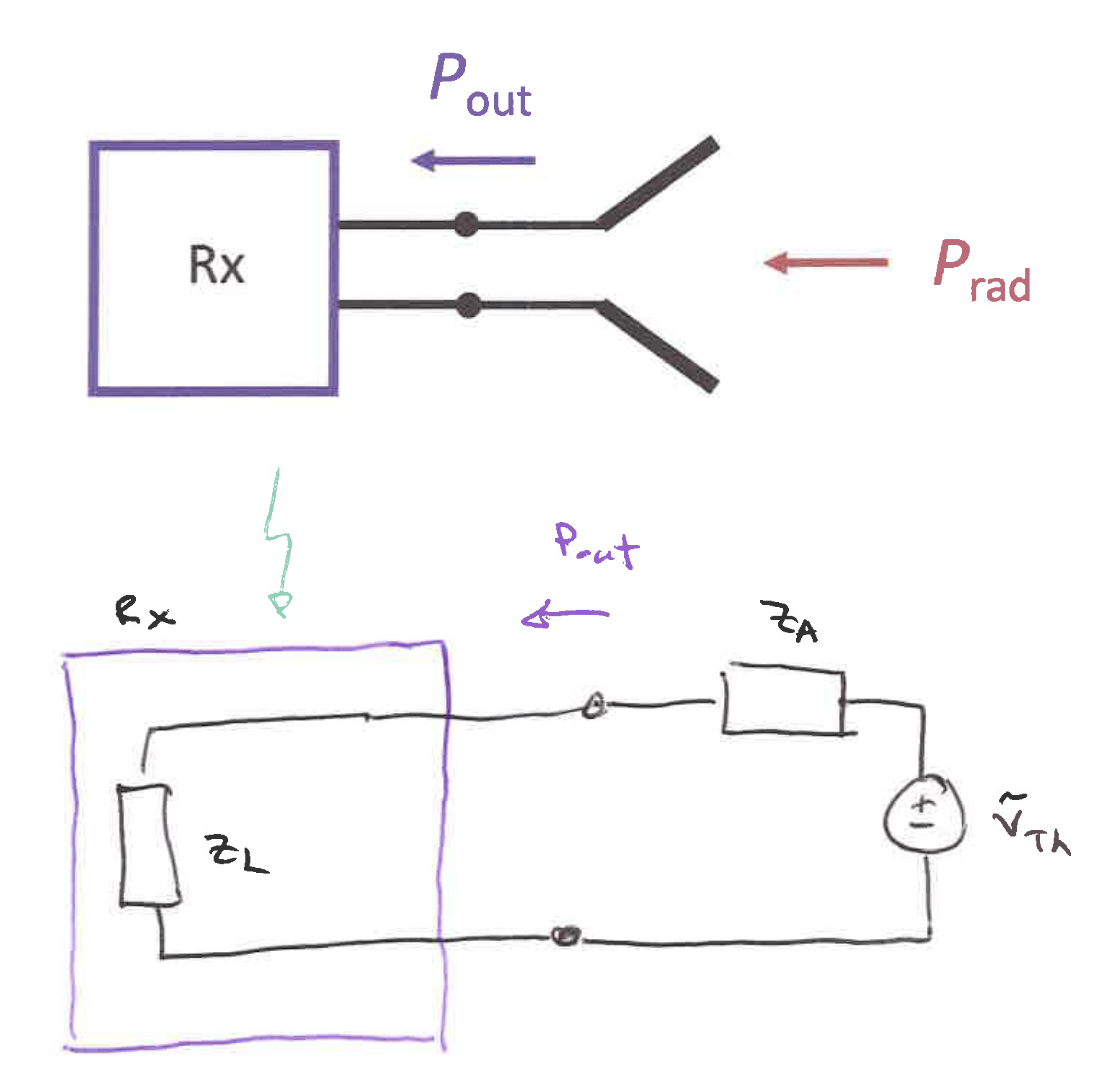
\includegraphics[width=1\textwidth]{./image/figure6.png}
    \caption{Thevenin Equivalent of Receiver with Antenna as Transmitter}
\end{figure}

\begin{quote}
    Our goal is to have the antenna's power fully dissipated by $Z_L$.
    This is an identical problem as optimizing $P_{in}$. Therefore,

    \[Z_g = Z_A^*\]

    In this case, $P_{out}$ is
    \[P_{out} = \frac{1}{2}|\tilde{I}|^2 R_A = \frac{1}{2}\left(\frac{|\tilde{V}_{TH}|}{2R_A}\right)^2R_A = \frac{|\tilde{V}_{TH}|^2}{8R_A}\]
\end{quote}

\subsection{Thevenin Voltage of the Antenna}
\begin{figure}[H]
    \centering
    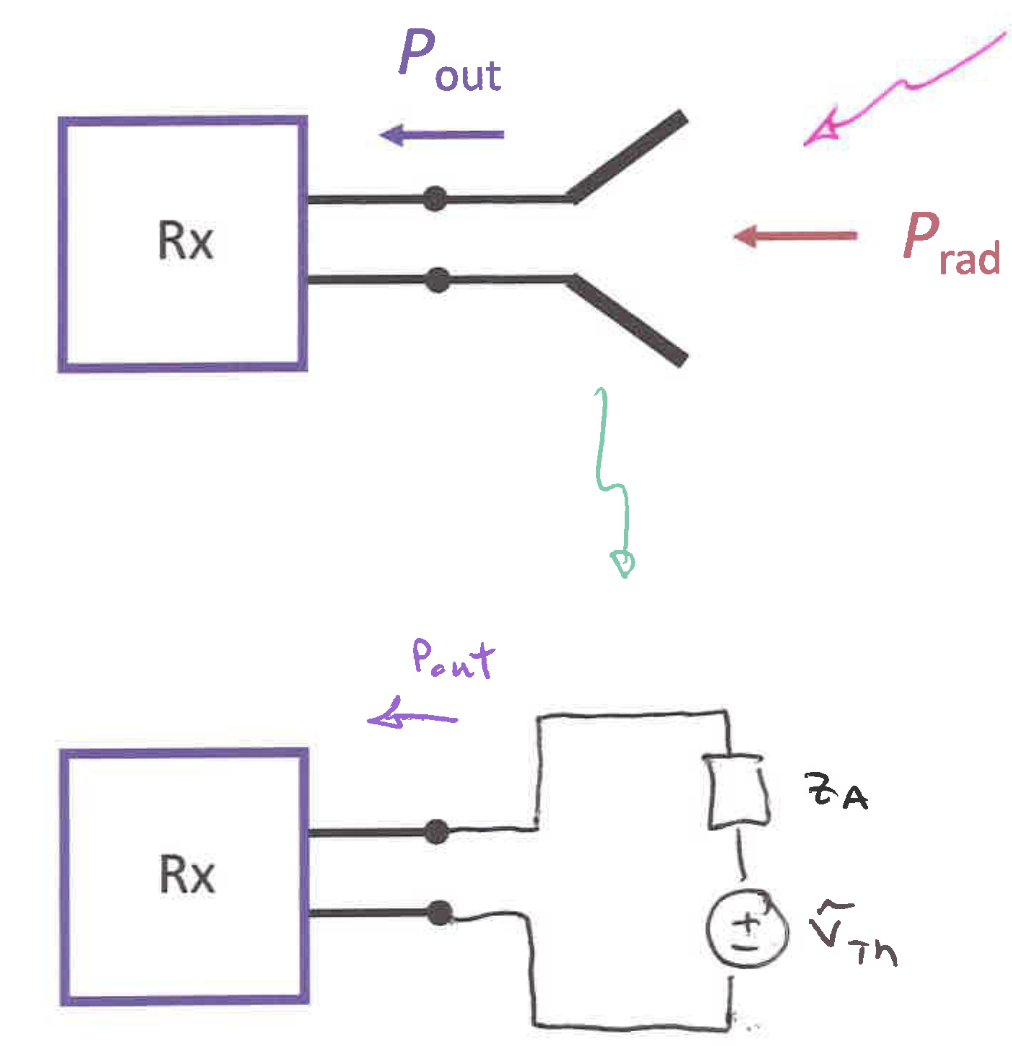
\includegraphics[width=0.5\textwidth]{./image/figure7.png}
    \caption{Thevenin Voltage of Antenna}
\end{figure}
\begin{quote}
    Power delivered to a matched load with a lossless antenna

    \[P_{out} = A_e S_i\]

    \[\frac{|\tilde{V}_{TH}|^2}{8R_A} = A_e S_i\]

    \[|\tilde{V}_{TH}| = \sqrt{8 R_A A_e S_i}\]
\end{quote}

\section{Antenna Links}

\begin{figure}[H]
    \centering
    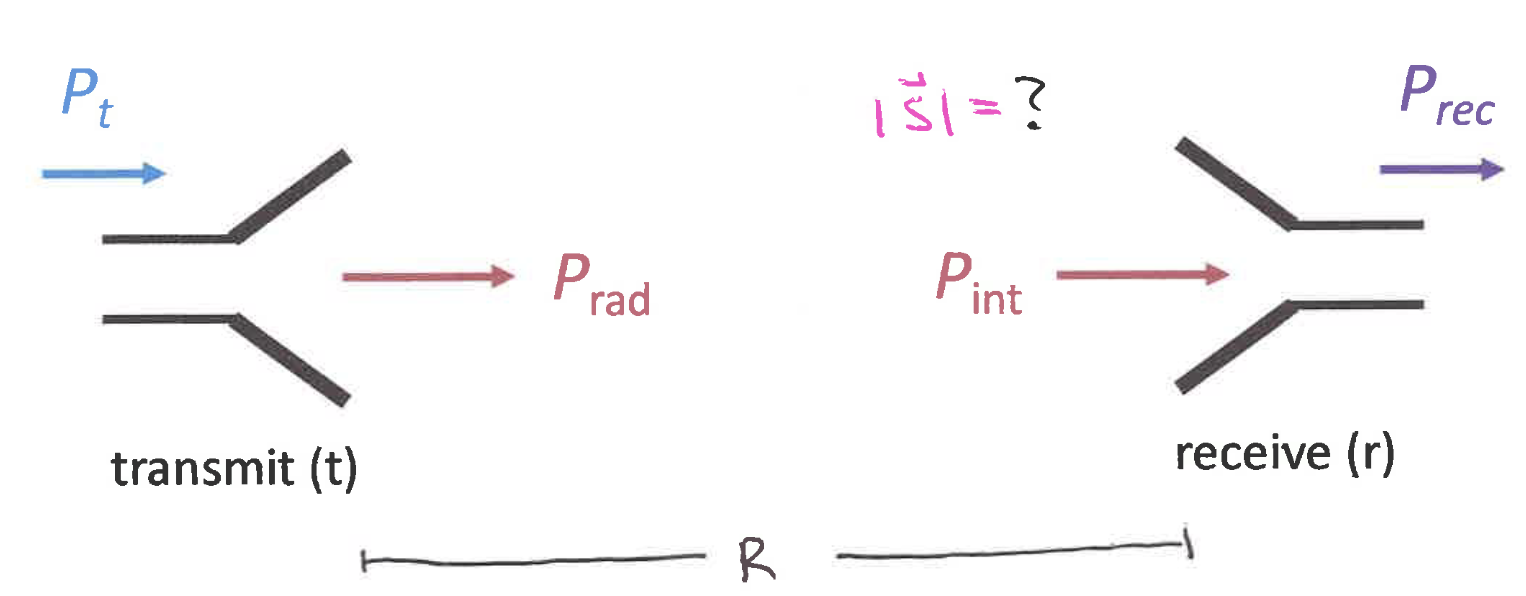
\includegraphics[width=1\textwidth]{./image/figure8.png}
    \caption{Antenna Link}
\end{figure}

\begin{quote}
    When one antenna transmits a signal to the other antenna, the power ratio between the transmitter and the receiver could be modeled by the \textbf{Friis Transmission Equation}.

    \[\frac{P_{rec}}{P_{t}} = e_r e_t \left(\frac{\lambda}{4\pi R}\right)^2 D_r D_t\]
    \[= \frac{e_r e_t A_r A_t}{\lambda^2 R^2}\]

    where $A_r$, $A_t$ are the effective area of the antenna, $e_r, e_t$ are the efficiency of the antenna, $\lambda$ is the wavelength of the transmitted wave, and $D_r, D_t$ are the directivity of the antennas.


\end{quote}

\begin{quote}
    The signal to noise ratio: $10 \log\left(\frac{P_{\text{receive}}}{P_{\text{noise}}}\right)$
\end{quote}

\section{Maxwell's Equation}
\begin{quote}
    % Add the differential version

    The divergence of E field is proportional to enclosed charge because more charges produces more E field.

    $$\nabla \cdot \vec{E} = \frac{\rho}{\epsilon}$$

    $$\oint \vec{E} \cdot d\vec{A} = \frac{Q_{enclosed}}{\epsilon_0}$$


    The divergence of H field is zero because there's no magnetic monopole. H field will enter and leave at every point.

    $$\nabla \cdot \vec{H} = 0$$

    $$\oint \vec{B} \cdot d\vec{A} = 0$$

    The curl of the E field is zero in static case, just like Kirchhoff's Voltage law that sums the voltage to 0. The dynamic case shows that the curl is proportional to the change in magnetic flux through the loop.

    $$\nabla \times \vec{E} = -\mu \frac{\partial \vec{H}}{\partial t}$$

    $$\oint \vec{E} \cdot d\vec{l} = -\frac{d\phi_B}{dt}$$

    The curl of the H field is proportional to the current density plus the change in E flux through the loop.

    $$\nabla \times \vec{H} = \epsilon \frac{\partial \vec{E}}{\partial t}$$

    $$\oint \vec{B} \cdot d\vec{l} = \mu_0 i + \mu_0 \epsilon_0 \frac{d \phi_E}{dt}$$
\end{quote}

\subsubsection{Inhomogeneous Wave Equation}
\begin{quote}
    When we construct the wave equation with Maxwell's Equation with source, we get
    \[\nabla^2\vec{E}-\mu_0\epsilon_0 \frac{\partial ^2}{\partial t^2}\vec{E} = \nabla\left(\frac{\rho}{\epsilon_0}\right) + \mu_0 \frac{\partial}{\partial t} \vec{J}\]

    We can think of the left hand side of the equation as a system created by physical laws, and the right hand side as the input to the system. After the input (charges and currents) is applied, the system will output some E field.

    It's similar to the motion of a spring and mass system.

    \begin{figure}[H]
        \centering
        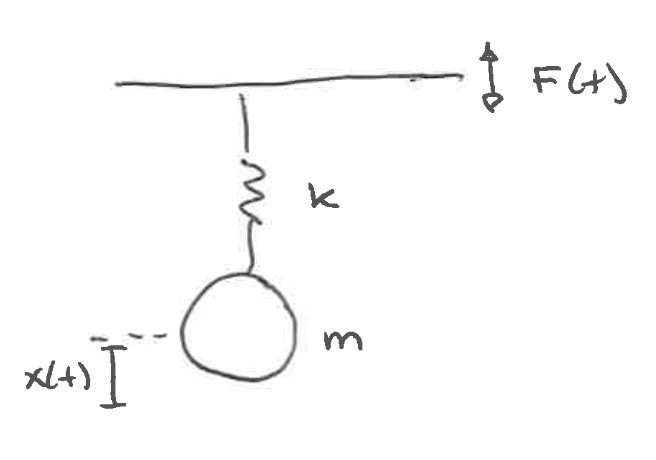
\includegraphics[width=0.5\textwidth]{./image/figure4.png}
        \caption{Spring-Mass System}
    \end{figure}

    \[m \frac{d^2 x}{dt^2} = -kx -bv + F(t)\]

    By rearranging the terms, we get

    \[m \frac{d^2 x}{dt^2} + b\frac{dx}{dt} + kx = F(t)\]

    Notice that the left hand side is a system that spits out the position of the mass, and the right hand side is the applied input force.
\end{quote}

\subsection{Vector Potential and Gauges}
\begin{quote}

    We define the \textbf{vector potential}, $\vec{A}$, as
    \[\vec{B} = \nabla \times \vec{A}\]

    Since $\nabla \times \vec{E} = - \frac{\partial \vec{B}}{\partial t}$




    \[\vec{E} = - \nabla \phi - \frac{\partial \vec{A}}{\partial t}\]

    where $\phi$ is the electrostatic potential.

    \bigskip
    As a result, the H and E field can be written in terms of the \textbf{Vector Potential}

    \[\vec{H} = \frac{1}{\mu_0} \nabla \times \vec{A} \]

    \[\vec{E} = -\nabla\phi - \frac{\partial \vec{A}}{\partial t}\]

\end{quote}
\subsection{Interesting Property}
\begin{quote}
    \[\vec{A}_{new} = \vec{A} + \nabla\psi\]

    Curl both sides

    \[\frac{1}{\mu_0}\nabla \times \vec{A}_{new} = \frac{1}{\mu_0}\nabla \times \vec{A} + \frac{1}{\mu_0}\nabla \times \nabla\psi\]

    Notice

    \[\vec{H}_{new} = \vec{H}\]

    In the case of an E field,

    If $\phi_{new} = \phi - \frac{\partial \psi}{\partial t}$, then $\vec{E}_{new} = \vec{E}$

    \bigskip
    In summary,

    \[\phi_{new} = \phi - \frac{\partial \psi}{\partial t}\]

    and

    \[\vec{A}_{new} = \vec{A} + \nabla\psi\]

    implies

    \bigskip
    E and H field produced by $\phi_{new}$ and $\vec{A}_{new}$ are same as those made by $\phi$ and $\vec{A}$
\end{quote}

%Rewrite the inhomogeneous wave equation with the vector potential

\section{Retarded Potential}

\section{The Hertzian Dipole}
\begin{quote}
    \subsection{Basics of Hertzian Dipole}
    \begin{itemize}
        \item A very short ($l \leq \frac{\lambda}{50}$) infinitesimally thin, wire carrying a uniform current.
    \end{itemize}

    $\vec{J}(\vec{r'}) = I_0 \delta(x)\delta(y)$

    Recall that we are in sinusoidal steady state.

    \[\rho(\vec{r}, t) = \Re \{\tilde{\rho}(\vec{r})e^{j \omega t}\}\]

    \[\vec{J}(\vec{r}, t) = \Re \{\tilde{J}(\vec{r})e^{j \omega t}\}\]

    Procedure to find the Antenna Parameters of the Hertzian Dipole
    \begin{enumerate}
        \item Calculate $\tilde{A}(\vec{r})$ using retarded potentials.
              \[\tilde{A} = \frac{\mu_0}{4 \pi}\int \frac{\vec{J}(\vec{r'})}{R}e^{-jkR}dV'\]
              Since R = r and is approximately constant every point on the wire,
              \[= \frac{\mu_0}{4 \pi}\frac{e^{-jkr}}{r} \int \vec{J}(\vec{r'})dV'\]
              \[= \frac{\mu_0}{4 \pi}\frac{e^{-jkr}}{r}\int \int \vec{J}(\vec{r'})  I_0 \delta(x)\delta(y) \cdot d\vec{A} dz\]
              \[\frac{\mu_0}{4 \pi}\frac{e^{-jkr}}{r}\int_{\frac{-l}{2}}^{\frac{l}{2}}I_0 \vec{z} dz\]
              \[= \frac{\mu_0 I_0 l}{4 \pi}\frac{e^{-jkr}}{r}\vec{z}\]
              \[= \frac{\mu_0 I_0 l}{4 \pi}\frac{e^{-jkr}}{r}(\cos(\theta) \hat{r} -\sin(\theta) \hat{\theta})\]
        \item Find H and E fields from $\tilde{A}(\vec{r})$.

              \bigskip
              Taking the curl in spherical coordinate
              \[\tilde{H} = \frac{1}{\mu_0}\frac{\mu_0 I_0 l e^{-jkr}}{4 \pi}\left(\frac{j}{kr} + \frac{1}{(kr)^2}\right)\sin(\theta)\hat{\phi}\]
              % Miss a term
              \[\tilde{E}= \frac{I_0 l k^2}{4 \pi}\eta_0 e^{-jkr}(\left(\frac{1}{kr} - \frac{j}{(kr)^3}\right)2\cos(\theta)\hat{\phi}) \]
        \item Break the H and E field into Near and Far Fields.

              \bigskip
              E field looks very complicated, so we will define two regions of $kr$ that simplifies the expression

              \bigskip
              Near Field: $kr << 1 \implies \frac{2 \pi}{\lambda} r << 1$
              \[\tilde{H}_{nF} = \frac{I_0 l}{4 \pi r^2}\sin(\theta) \hat{\phi}\]
              \[\tilde{E}_{nF} = \frac{q l}{4 \pi \epsilon_0 r^3}(2 \cos(\theta) \hat{r} + \sin(\theta) \hat{\theta})\]

              Notice that it looks like an electrostatic dipole

              \bigskip
              Far Field: $kr >> 1$ (generally what we care about)
              \[\tilde{H}_{FF} = \frac{\tilde{E}_{FF}}{\eta_0}\hat{\phi}\]
              \[\tilde{E}_{FF} = j\eta_0\frac{I_0 l k^2}{4 \pi} e^{-jkr}\sin(\theta)\hat{\theta}\]

        \item Find $\vec{S}_{avg}$ and antenna parameters.
              \[\vec{S}_{avg} = \frac{1}{2}\Re\{\tilde{E} \times \tilde{H}\}\]
              \[= \frac{1}{2 \eta_0} |\tilde{E}_{FF}|^2 \hat{r}\]


              Therefore,
              \[| \vec{S}_{avg} | = \frac{1}{2 \eta_0} \left(\eta_0 \frac{Ilk}{4 \pi r}\sin(\theta)\right)^2 = \frac{15 \pi I_0 ^2}{r^2}\left(\frac{l}{\lambda}\right)^2 \sin^2(\theta)\]
    \end{enumerate}
\end{quote}

\subsection{Hertzian Dipole's Antenna Parameter}
\begin{quote}
    We knew that the power radiated would be $\frac{1}{r^2} U(\theta, \phi)$. Therefore, the \textbf{radiation intensity} of a Hertzian Dipole is
    \[15 \pi I_0 ^2\left(\frac{l}{\lambda}\right)^2 \sin^2(\theta\]

    and the \textbf{normalized radiation intensity} is

    \[F(\theta, \phi) = \sin^2(\theta)\]

    The \textbf{total radiated power} is

    \[P_{rad} = \int U(\theta, \phi) d\Omega = \frac{8 \pi}{3}\]

    The \textbf{directivity pattern} is

    \[D(\theta,\phi) = \frac{U(\theta, \phi)}{\frac{P_{rad}}{4 \pi}} = 1.5 \sin^2(\theta)\]

    The \textbf{directivity} is $D_0 = 1.5$.

    When the circuit model of a Hertzian Dipole Antenna is lossless, the radiation loss equals the $R_{rad}$ of the antenna's equivalent resistance, which isotropic
    \[R_{rad} = 80 \pi^2 \left(\frac{l}{\lambda}\right)^2\]

    Since $l < \frac{\lambda}{50}$ for the Hertzian Dipole Antenna,
    \[R_{rad} < 80 \pi^2 \left(\frac{1}{50}\right)^2 = 0.32 \Omega\]

    We can see that the radiation resistance is very small, which could make it hard to match the resistance because the characteristic impedance of a transmission line is much larger.

    Effective area of the antenna is

    \[A_e = \frac{P_{int}}{S_i}\]

    When the antenna receives signal, the lossless condition implies that all intercepted power

    \[A_e = \frac{P_{int}}{S_i} = \frac{1}{8}\frac{|\tilde{V}_{oc}|^2}{R_{rad}} \frac{2 \eta_0}{|\tilde{E_i}|^2}\]

    Since,

    \[|\tilde{V}_{oc} | \approx | \tilde{E}_i|\], we have

    \[A_e = \frac{3}{8 \pi} \lambda^2\]


\end{quote}

\section{Small Dipole Antenna}

\begin{quote}
    The short dipole antenna has no current at the ends of the antenna, unlike the Hertzian Dipole Antenna (HD Antenna) with constant current everywhere.

    If we follow the steps of calculating vector potential of the HD Antenna, we will find that $\tilde{A}$ is half of that of the HD Antenna. Thus, the small dipole antenna gives half of the E and H fields compared to the HD Antenna.

    \[l \leq \frac{\lambda}{10}\]

    \[\tilde{A} = \left(\frac{1}{2}\right)\frac{\mu_0 I_0 l}{4 \pi}\frac{e^{-jkr}}{r}(\cos(\theta) \hat{r} -\sin(\theta) \hat{\theta})\]

    \[U(\theta, \phi) = \frac{15 \pi I_0 ^2\left(\frac{l}{\lambda}\right)^2}{4} \sin^2(\theta)\]

    \[P_{rad} = \]

    \[D(\theta, \phi) = 1.5 \sin^2(\theta)\]

    \[R_{rad} = 20 \pi^2 \left(\frac{l}{\lambda}\right)^2\]

    \[A_e = \frac{3 \lambda ^2}{8 \pi}\]
\end{quote}

\section{Finite Dipole Antenna}
\begin{quote}
    Current goes to 0 at the end of the pole. There's a standing wave current pattern on the poles.
\end{quote}

\section{Physical Intuition on Radiation}
\subsection{Why Transmission Line doesn't Radiate Wave}

\section{What Makes a Good Antenna?}
\begin{itemize}
    \item Good Radiation Pattern
    \item Good matching (nice circuit properties)
\end{itemize}


\end{document}
